 \documentclass{beamer}

\usetheme{MagdeburgFIN}
\usefonttheme{structurebold}
\usepackage{graphicx}
\usepackage{float}
\usepackage{url}
\usepackage{pdfpages}
\usepackage[ngerman]{babel}
\usepackage{lmodern}


\title{Performance Factors for Deep Learning and Shallow Neural Network Applications: \\ A Beginners Guide}
\author{Johannes W\"{u}nsche}
\date{\today}
\institute{}

\begin{document}

\begin{frame}[plain]
 \titlepage
\end{frame}



\section[Agenda]{}
\begin{frame}
\frametitle{Agenda}
\tableofcontents
\end{frame}

\section{Motivation}
\begin{frame}
\frametitle{Motivation}
\centering
\begin{tabular}{c c}
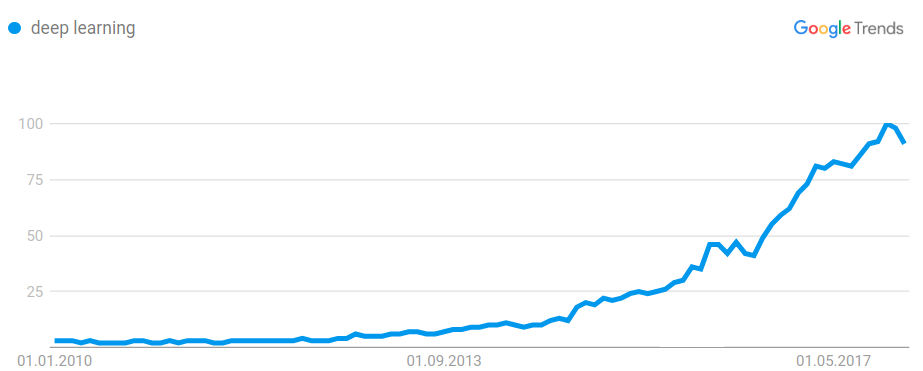
\includegraphics[width=0.5\textwidth]{pop.png} \\\\ 
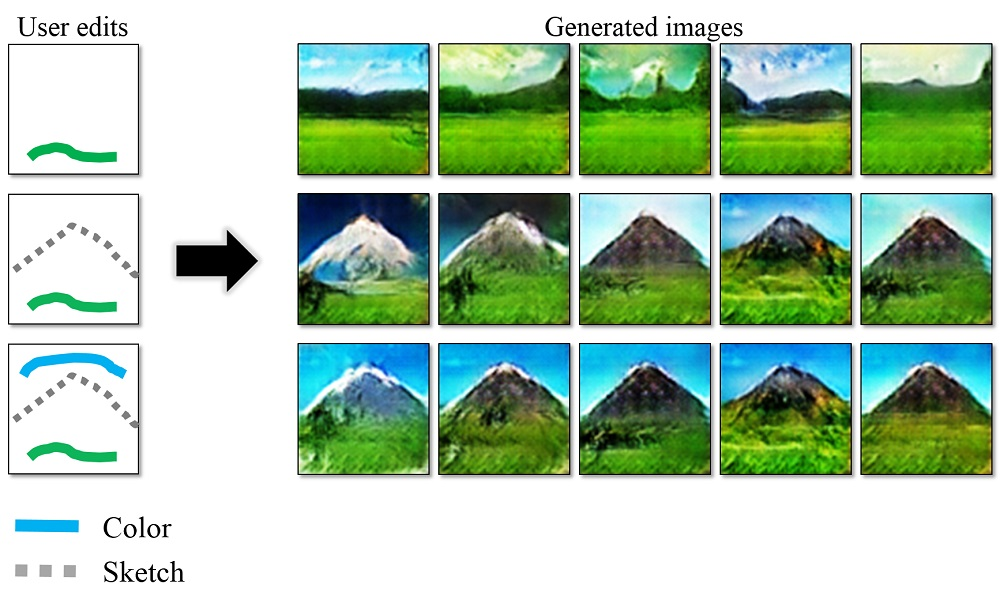
\includegraphics[width=0.5\textwidth]{demo_teaser.jpg}

 
\end{tabular}
\end{frame}



\section{Overview}
\begin{frame}
\frametitle{Overview}
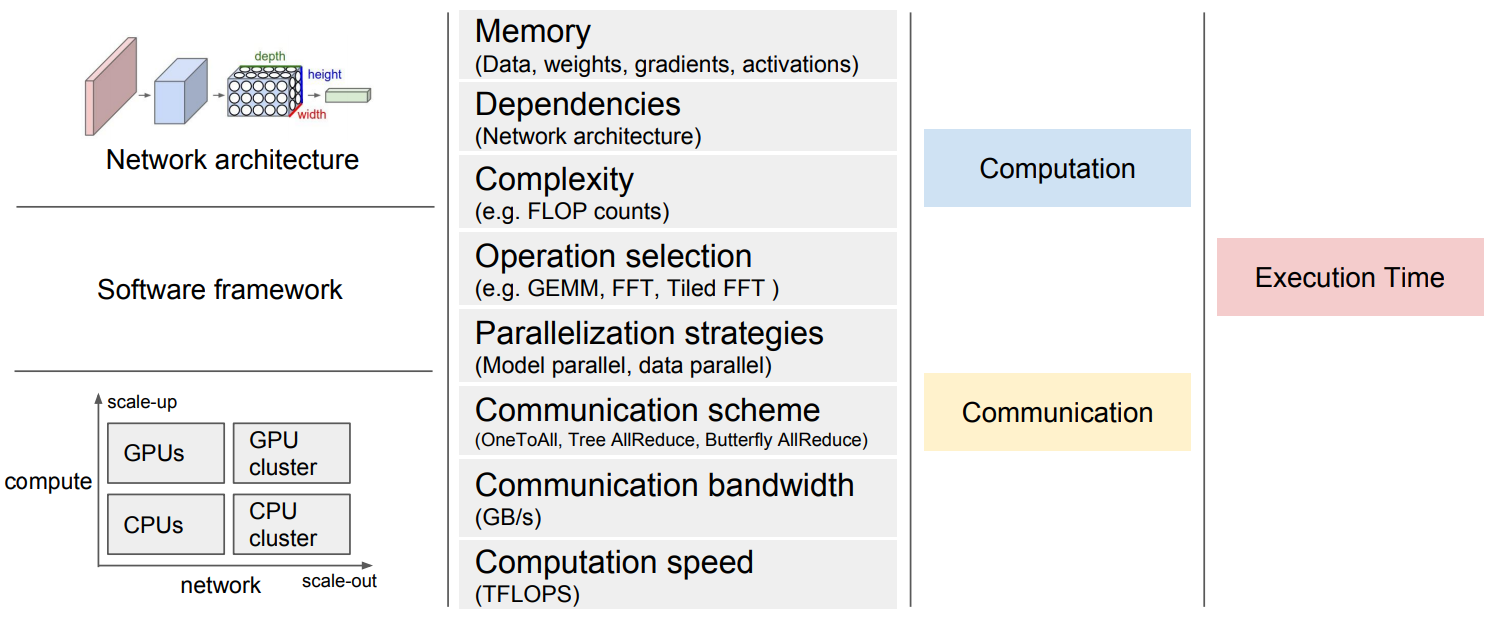
\includegraphics[width=\textwidth]{PaleoModel.png}
\end{frame}


\section{Choice of Neural Network}
\begin{frame}
\frametitle{Choice of Neural Network}
\begin{itemize}
\item Shallow Networks
\begin{itemize}
\item FFN, AE, RBM
\end{itemize}
\item Deep Networks
\begin{itemize}
\item VAE, DBN, GAN, RNN e.g. LSTM, DCN, DN, RN
\end{itemize}
\item Hyperparameters
\item Usage of specific networks
\end{itemize}
\end{frame}

\begin{frame}
\centering
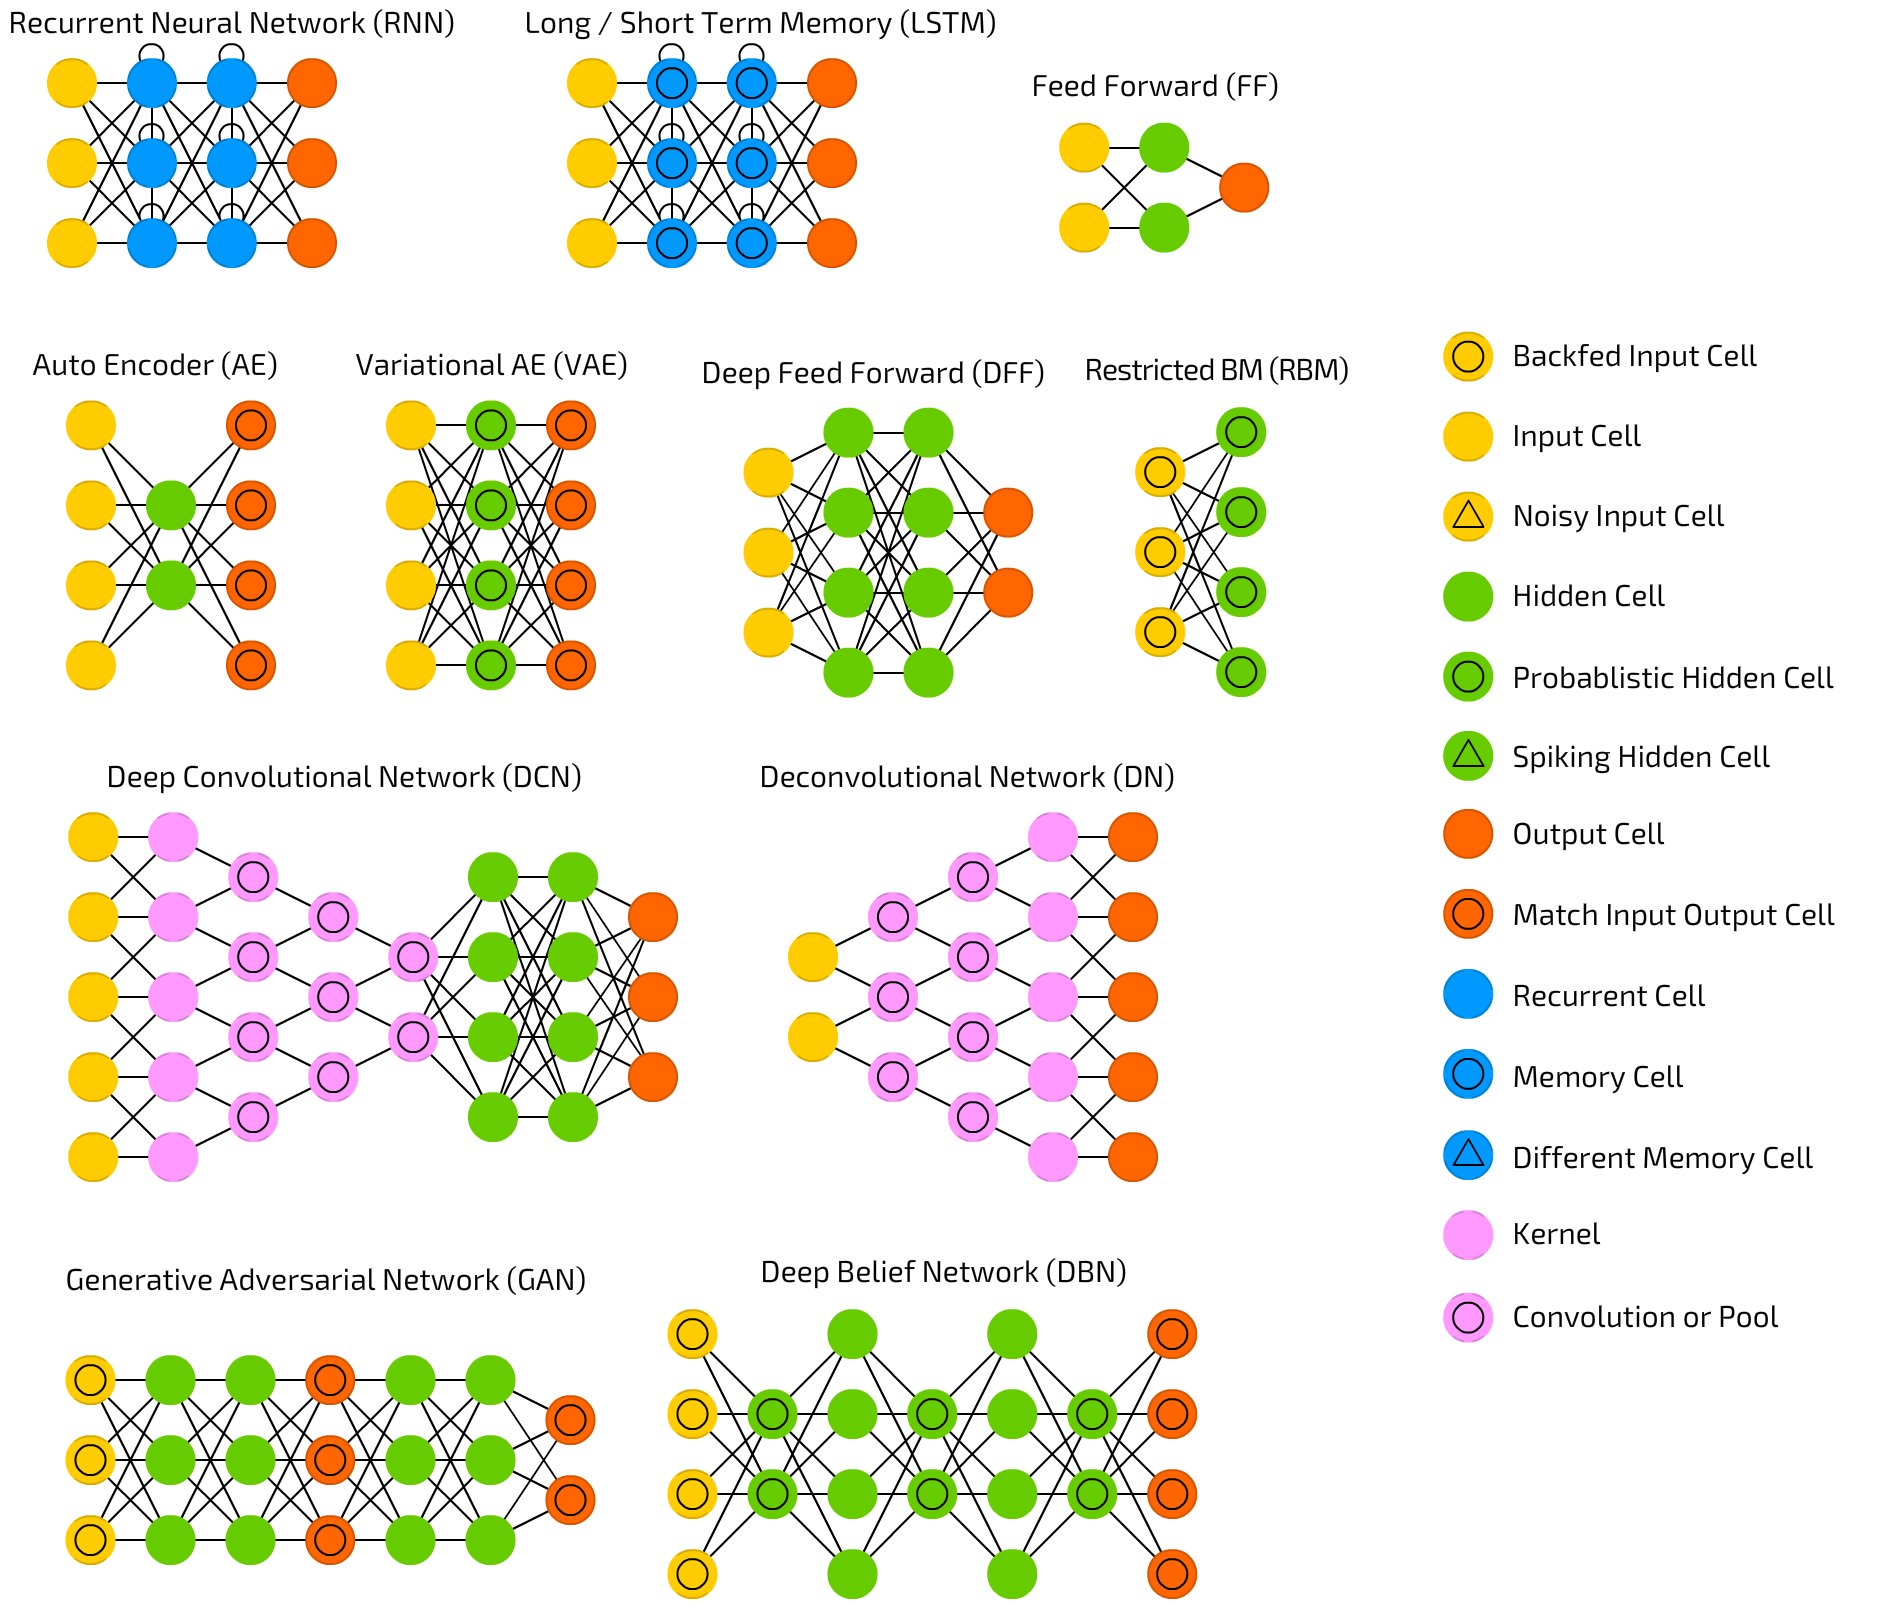
\includegraphics[height=\textheight]{neuralnetworks.png}
\end{frame}

\section{Choice of Processing Unit}
\begin{frame}
\frametitle{Choice of Processing Unit}
\begin{itemize}
\item CPU
\begin{itemize}
\item Single-thread
\item Multi-thread
\item Advantage
\item Disadvantage
\end{itemize}
\item GPU
\begin{itemize}
\item Single unit
\item Multi-GPU
\item Advantage
\item Disadvantage
\end{itemize}
\item GPU-Cluster
\begin{itemize}
\item Advantage
\item Disadvantage
\end{itemize}
\end{itemize}
\end{frame}

\begin{frame}
\begin{tabular}{c c}
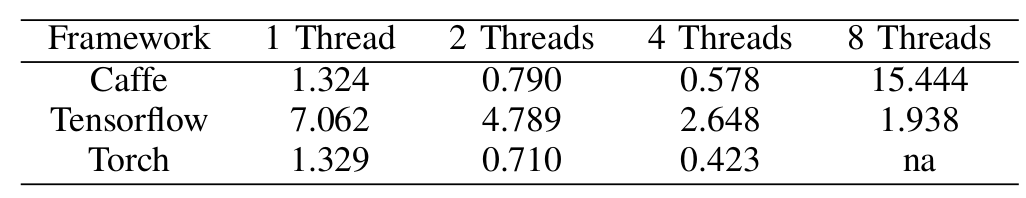
\includegraphics[width=0.4\textwidth]{table.png} &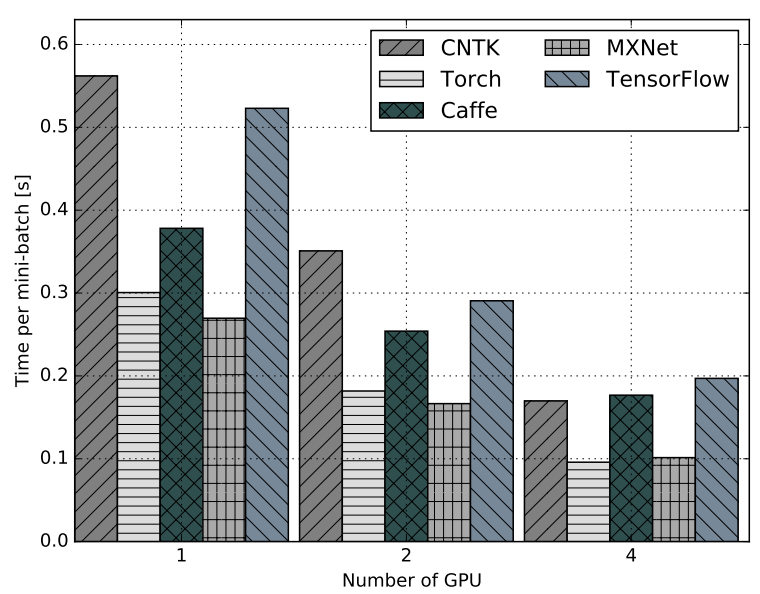
\includegraphics[width=0.4\textwidth]{a.png} \\
\end{tabular}
\centering
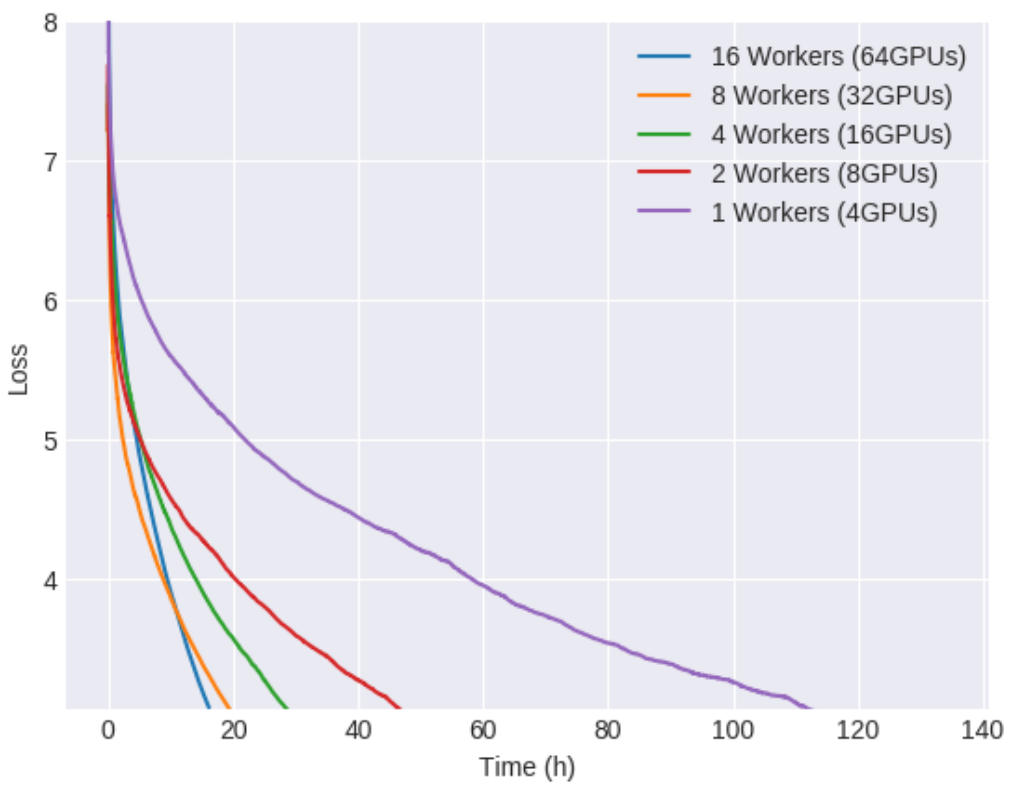
\includegraphics[width=0.4\textwidth]{gpu_cluster_perf_win.png}
\end{frame}

\section{Challenges}
\begin{frame}
\frametitle{Challenges}
\centering
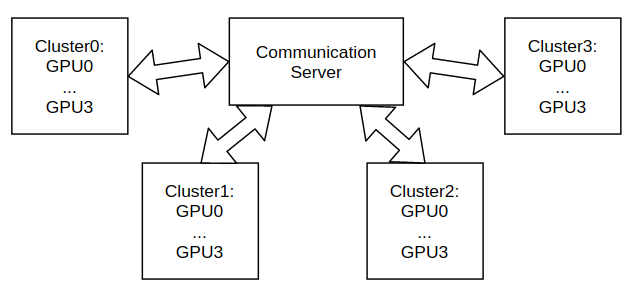
\includegraphics[width=0.8\textwidth]{cluster_setup.png}

\end{frame}

\begin{frame}
 \frametitle{Thank you for your attention!}
\end{frame}

\begin{frame}[allowframebreaks]
\frametitle{References}
\nocite{*}
\tiny
\bibliographystyle{IEEEtran}
\bibliography{paper}
\end{frame}


\end{document}
